%
% File acl2021.tex
%
%% Based on the style files for EMNLP 2020, which were
%% Based on the style files for ACL 2020, which were
%% Based on the style files for ACL 2018, NAACL 2018/19, which were
%% Based on the style files for ACL-2015, with some improvements
%%  taken from the NAACL-2016 style
%% Based on the style files for ACL-2014, which were, in turn,
%% based on ACL-2013, ACL-2012, ACL-2011, ACL-2010, ACL-IJCNLP-2009,
%% EACL-2009, IJCNLP-2008...
%% Based on the style files for EACL 2006 by 
%%e.agirre@ehu.es or Sergi.Balari@uab.es
%% and that of ACL 08 by Joakim Nivre and Noah Smith

\documentclass[11pt,a4paper]{article}
\usepackage[hyperref]{acl2021}
\usepackage{times}
\usepackage{latexsym}
\renewcommand{\UrlFont}{\ttfamily\small}
\usepackage{graphicx}

% This is not strictly necessary, and may be commented out,
% but it will improve the layout of the manuscript,
% and will typically save some space.
\usepackage{microtype}

\aclfinalcopy % Uncomment this line for the final submission
%\def\aclpaperid{***} %  Enter the acl Paper ID here

%\setlength\titlebox{5cm}
% You can expand the titlebox if you need extra space
% to show all the authors. Please do not make the titlebox
% smaller than 5cm (the original size); we will check this
% in the camera-ready version and ask you to change it back.

%\newcommand\BibTeX{B\textsc{ib}\TeX}


\usepackage{biblatex} %Imports biblatex package
\addbibresource{Shakespeare Text Generation.bib} %Import the bibliography file
%\addbibresource{sample.bib}

\title{Shakespearean Text Generation Report}
\author{  R. Chen (\textit{rc29@pdx.edu}) \and F. Pearson (\textit{fpearson@pdx.edu})\\ \textbf{J. Ressler (\textit{jressler@pdx.edu})} \and \textbf{E. Weisman (\textit{weisman@pdx.edu})}}

\begin{document}


%  \texttt{email@domain} \\\And
 % Second Author \\
  %Affiliation / Address line 1 \\
  %Affiliation / Address line 2 \\
  %Affiliation / Address line 3 \\
  %\texttt{email@domain} \\}

%\author{
%\begin{tabular}[t]{c@{\extracolsep{8em}}c} 
%R. Chen & F. Pearson & J. Ressler & E. Weisman 
%\end{tabular}
%}


\maketitle



\date{11/23/2022}

\begin{abstract}
Natural Language Processing has evolved in a multitude of way, and sees use in many facets of modern life. It also exists as a stark pillar of modernity within computer science. In contrast to this, the writings of William Shakespeare are iconic relics from a prior millennia. We asked the question: "Can current modern methods reproduce plausible results when attempting to extend Shakespeare's corpora?" In pursuit of this question, a model was built and used to provide a host of 'Shakespearean' text, which was evaluating by human elements, alongside other similar models, to evaluate the results in a non-biased manner. The process begins with the creation of a corpus of Shakespeare's plays, which are then used to generate new lines of dialogue in an attempt to reproduce the original wording as closely as possible. This technique has been applied successfully to his prose.

\end{abstract}

\section{Credits}
Ray helped with early prototyping of the model. His contributions to the presentation slide deck heavily focused on the results section. He helped revise and proofread the survey used for evaluating the model. Ray worked closely with Eben to compile the results of the model evaluation.\\
Forest Helped with prototyping the initial models found by the team initially. Also after prototyping he got the final tensorflow based GRU developed, setup, and running on the processed Shakespeare dataset. He also assisted in collecting results for the survey by advertising when applicable. Worked on the technical portions of the slidedeck as well as the paper itself covering the GRU.\\
James helped to find and prepare the dataset from selected plays by Shakespeare. He also tested out early prototypes of the model and collected documentation on how to build said model. He formulated the survey for evaluating the model. James, along with everyone on the team, contributed to all parts of the presentation slide deck and James focused heavily on the insights and ethical considerations sections. Similar contributions were made to the project report.\\
Eben helped with initial conceptualizing, and some preliminary research. He also did work with the questionnaire: Finding, and filling other models for comparison; compiling and formatting data; building graphics for the group presentation. Eben’s work on the presentation focused mostly on his presented sections: Introduction; explication of models, NLP tasks, and evaluation practices. His contributions to the paper were the introduction, and overview. Finally he helped with editing the paper, and transcribing it to LaTex.

\section{Introduction}
\label{sec:intro}
We have spent our time with the development of a natural language generator, with the explicit purpose of generating legible text in a Shakespearean format. We set out with the goal of answering the question: Can AI write like Shakespeare? To accomplish this, we built a model, with guidance from multiple online sources to generate text, based off of a brief prompt. The AI model then outputs what it believes to be appropriate characters and words, to form Shakespearean text. When building the generation model, we attempted both a LSTM and GRU approach. In the end we opted to go with the GRU approach, as it had an expedient run-time and produced seemingly superior results. In order to test the validity of our model, we implemented a brief questionnaire using google forms, which was supplied to peers, friends, and family. In this questionnaire, we posed various texts, either from Shakespeare himself, or generated by our, or another, model. The respondents were not given information on the source of the texts. The respondents were then asked to rate the given text on a scale of one to ten, with one being the least like Shakespeare and ten being the most like Shakespeare.\\
In the pages to follow, we evaluate and explicate our data, and will determine the success of both our model in comparison to the others, as well as to the source material. Following this, we evaluate the general success text generation on producing Shakespearean English. As an added exercise, we examined text generated based on other creative commons literature using our model, although this was not evaluated on a large scale.

\section{Process Breakdown}
\label{sec:process}
\subsection{Our NLP Task}
Our project aims to address the NLP task of text generation. Specifically, generating text that imitates Shakespeare’s writing. We trained a model on a combination of excerpts from several of Shakespeare’s comedies. The model accepts a seed string as input. The outputs are novel excerpts that appear to be written by Shakespeare but are completely original. For example, if we provide the input string “COUNTESS” then the output follows:  \\
\linebreak
“COUNTESS \\
To be young again, if we could: I will be a fool\\
Which he fains my thoughts Indeed.”\\
\linebreak\\
We can consider that output as successful if it can reliably pass as Shakespeare to a random reader. Even if the output cannot fool a reader in a direct comparison, the text should still resemble the Shakespearean form.

\subsection{Our Dataset}
\label{sec:data}
The datasets we made use of throughout this project were predominantly Shakespearean works\cite{complete} as well as some Jane Austen for comparison. This was due to the nature of this project being text generation; sourcing public works of well respected literature was a key principle for building our model. The collected files were then processed into text files for ease of use with our TensorFlow\cite{tensor} model. Our Shakespeare dataset consisted of three separate works totaling \textbf{72,742} words. These works were: All’s Well That Ends Well, As You Like, and Winter's Tale. These texts were chosen predominantly due to them all being comedies among Shakespeare's works, allowing us to get a larger sample size without diverting into excessively different grammatical prose. The Jane Austen set was taken for similar reasons, but also to test a dataset with a stark grammatical contrast to our main project with its rather dry and precise grammar.

\subsection{Methodology}
\label{sec:method}
The model we predominantly made use of throughout the project was a gated recurrent unit (GRU) based recurrent neural network using TensorFlow\cite{tensor} tools and libraries to set it up. This was chosen after early testing among a variety of other RNN models, such as the traditional LSTM due predominantly to its ease of use, increased speed, and lessened processing demands. This allowed us to test our model on a wide variety of epochs and variables with relative ease. For implementation the model makes use of TensorFlow\cite{tensor} optimizers, loss functions, and layers. The importing and configuring of the dataset, along with the outputting of text was implemented on our end, albeit following the TensorFlow\cite{tensor_tutorial} documentation to ensure compliance in regards to formatting matrices.\\
With this model, we set up the methodology to import the formatted datasets, before testing them with appropriate variables regarding epochs, RNN units, embedding, and seeds, to determine what yielded the best results. This was done while comparing against other existing models and datasets available online, such as the Towards Data Science LSTM\cite{TDS_model} or John Fish’s GRU\cite{fish_johnafishshakespeare_ai_2022} system. Once this was finalized, our team created and distributed a survey consisting of results from our model, written Shakespeare, and the other two models, in order to gauge the accuracy of such generators when imitating Shakespeare.

\subsection{The Results}
\label{sec:results}
\begin{figure}
\centering
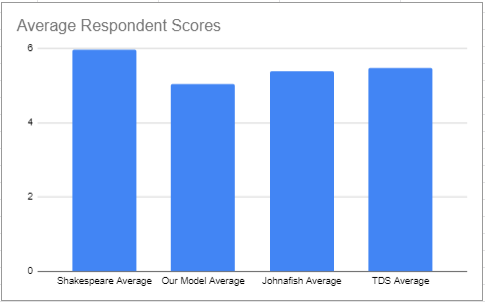
\includegraphics[width=.45\textwidth]{report/avgScores.png}
\caption{\label{fig:AverageScores}A bar chart showing the averages of scores by sources.}
\end{figure}
We compared our model’s texts to Shakespeare’s actual text, as well as the texts of the John Fish\cite{fish_johnafishshakespeare_ai_2022}, and Towards Data Science\cite{TDS_model} models as baselines to compare with. After our peers evaluated all thirty text samples on a score from 1-10 (least to most Shakespearean), we analyzed the samples’ scores in order to interpret results regarding their sources.\\
As can be observed through figure \ref{fig:AverageScores} our model performs slightly under (~7\%) the other two models. Given that the John Fish model operates on GRU and the Towards Data Science Model is using an LSTM, we can surmise that our under-performance is not necessarily due to model selection. That does not mean model choice was not a factor, as the lower average of the John Fish could hint to a slightly inferior performance from a GRU system. Our testing reflected this, however we chose a GRU system, as the impact to performance an LSTM had was not worth the slight increase to results we observed.\\ 
That said, all models performed similarly well, and not drastically behind the performance of Shakespeare's writings (functionally our control).\\
Figure \ref{fig:QuestionTotals} shows the total rating score received by each text sample, with their source being labeled across the x-axis. While at first glance this bar graph seems to imply middling results among the 4 text sources, there are some interesting things to note:
\begin{itemize}
    \item While many of the top percentiles for Question Totals belong to Shakespeare as the source, the fourth highest score was generated by our own model!
    \item Our model also produced its own outlier by way of having the lowest Question Total Score.
\end{itemize}
From these graphs and our analyses of them, we can conclude from these results that while our model is not crushing any expectations in comparison to the baselines that are set, our model still performs nearly on par with the John Fish and TowardsDataScience models, both of which are close to decently replicating the style of Shakespeares’ texts.\\ 
\begin{figure}
\centering
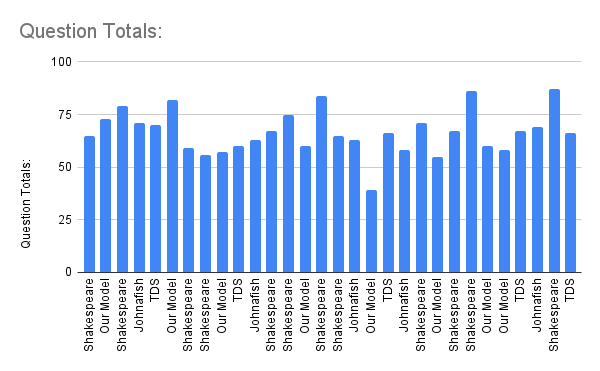
\includegraphics[width=.45\textwidth]{report/qTotals.png}
\caption{\label{fig:QuestionTotals}A bar chart showing the total score of each question.}
\end{figure}

\section{Interesting Insights}
\label{sec:insight}
The concept for this project took shape early in the term, however, the knowledge required to implement it did not arrive until later. A major problem with the model lay in the subtleties of coherence. At a glance, the model’s output appears Shakespearean in both cadence and form yet breaks down upon trying to derive any meaning from the generated passage. Had we more time, we would experiment more with fine tuning hyperparameters and perhaps even try restructuring the model altogether to include more advanced features.\\
The model did appear to blend in convincingly with genuine excerpts from Shakespeare. Some of this may be attributed to Shakespeare’s unique style, which serves to mask poor grammar and punctuation. At a shallow level, the model produces passable Shakespeare but the outputs do not hold up to strict scrutiny. 

\section{Ethical Considerations}
\label{ssec:ethics}
As cyberattacks become more commonplace, an often exploited attack vector is low- to mid-level employees, via social engineering and phishing. These tools have an obvious use in the hands of scam organizations that work on high volume; sending out mass emails in the hope that one employee opens it. Misuse of these technologies is a major concern in these well-defined cybercrime spaces and gives rise to a fundamental question of ownership: does an artist have claim to pieces produced by models trained on their original work? As these models become more convincing, artists may begin to see the circulation of work that bears their unique style. We have already started to see this phenomenon in digital art spaces and can easily imagine the rise of robot writers trained on the works of iconic individuals and well-known persons.\\

\section*{Acknowledgments}

We would like to thank Dr. Ameeta Agrawal, for time rendered teaching us, as well as a insight, and guidance. We also wish to thank Rhitabrat Pokharel, our wonderful TA. Along with each other, for a cohesive work experience. \\

\textbf{Source Code can be found on our GitHub\cite{pearson_cs410-510-nlp-project_2022}}\\
\textit{https://github.com/ForestPearson/CS410-510-NLP-project}

\nocite{*} 
\printbibliography[title={Bibliography}] 

%\bibliographystyle{acl_natbib}
%\bibliography{anthology,acl2021}

%\appendix



\end{document}
